\documentclass[10pt,onecolumn]{article}

\usepackage[a4paper,margin=1.65cm]{geometry}
\usepackage[T1]{fontenc}
\usepackage[utf8]{inputenc}
\usepackage{lmodern}

\usepackage{amsmath,amssymb,bm}
\usepackage{graphicx}
\usepackage{booktabs}
\usepackage{tabularx}
\usepackage{siunitx}
\usepackage{caption}
\usepackage{subcaption}
\usepackage{xcolor}
\usepackage{cite}
\usepackage{placeins}

\usepackage{setspace}
\usepackage{indentfirst}

\usepackage[colorlinks=true, citecolor=blue, linkcolor=blue, urlcolor=blue]{hyperref}

\onehalfspacing
\setlength{\parindent}{1.25cm}
\setlength{\parskip}{0pt}

\usepackage{authblk}

\renewcommand\Authfont{\normalsize}
\renewcommand\Affilfont{\small}
\setlength{\affilsep}{0.35em}

\captionsetup{
  font=small,
  labelfont={bf,color=blue}
}

\sisetup{detect-all=true}

\title{Learning quantum eigenspaces under geometric symmetry breaking with Rayleigh--Ritz physics-informed neural networks}

\author[1]{Leonardo dos Santos Vitoria}
\author[2]{Mikael Alcantra}
\author[2]{Gregório Candido dos Santos Valadares de Almeida}
\author[2]{Daniela Cristina da Silva Rodrigues Vitoria}
\author[2]{Gilvan de Jesus Pirôpo}

\affil[1]{Laboratório de Materiais Avançados e Minerais Estratégicos -- LMM,\\
Universidade Federal de Lavras (UFLA), Lavras, MG, Brazil}
\affil[2]{Universidade Federal de Sergipe (UFS), São Cristóvão, SE, Brazil}

\date{\today}

\begin{document}

\maketitle

\begin{abstract}

We develop a Rayleigh--Ritz physics-informed neural formulation for quantum eigenproblems on geometry-parametrized domains, in which the neural representation and its validation diagnostic track the spectral object selected by the physics rather than the eigenvalue index alone. Tested on the one-dimensional well, the square-to-rectangle and disk-to-ellipse deformations, and a controlled avoided crossing, the formulation recovers ordered excited states by explicit projection, degenerate eigenspaces by subspace Rayleigh--Ritz training without imposing a particular basis, symmetry-split branches by parity-adapted sectors, and near-degenerate bands by modal-overlap tracking. Two controls sharpen this picture: replacing the avoided-crossing potential with a purely geometric shear reproduces the same level repulsion, showing that the effect is generic to geometric coupling rather than an artifact of the added potential; and a pointwise-residual baseline succeeds only when initialized near the target energy, collapsing onto the wrong state otherwise, unlike the projection-based formulation, which requires no such prior. These results give a practical diagnostic hierarchy for neural eigensolvers of Hermitian operators under geometric deformation.

\end{abstract}

\section{Introduction}

When an electron is confined to a very small region of space, the geometry of that region becomes part of the quantum problem. The allowed energies are no longer determined only by the material or by the depth of the confining potential, but also by the size, shape, dimensionality, and boundary of the confinement domain. In realistic semiconductor quantum dots, this geometric control of confined levels is one of the reasons why such systems are often described as artificial atoms: spatial confinement discretizes the spectrum, while the geometry controls how the discrete levels are arranged \cite{Kastner1993,Ashoori1996,Kouwenhoven2001,Reimann2002,Jacak1998,Reimann1997}. A related idea appears in spectral geometry, where the eigenvalues of a Laplace or Schrödinger operator carry information about the domain on which the operator acts \cite{Kac1966,Weyl1911,Balian1970,Fox1967,Kuttler1984}. In this sense, an ideal quantum dot provides a controlled setting for studying how eigenvalues, eigenfunctions, and eigenspaces reorganize when the confinement geometry is changed.

The basic physical mechanism is simple. Symmetry can create degeneracies, and geometric deformations that break the symmetry can lift those degeneracies into distinct spectral branches \cite{Tinkham1964,Sakurai2020,Kato1995,Courant1953,AraujoLima2023,Dietz2008,Ree1998}. The symmetry of the confinement domain therefore organizes the eigenspaces as well as the eigenvalues of the Hamiltonian. For example, in a square well, the eigenfunctions $\psi_{1,2}$ and $\psi_{2,1}$, labeled by the quantum numbers $(1,2)$ and $(2,1)$, have the same energy because the Hamiltonian is invariant under the exchange $x\leftrightarrow y$. In a circular disk, rotational symmetry produces angular doublets. When the square is deformed into a rectangle, or the disk into an ellipse, the symmetry is reduced and the degeneracy is lifted. One might be tempted to set these geometries aside as too elementary to be worth reporting, since none of them poses any real difficulty for a classical solver, yet that is exactly what makes them useful here, since the relevant spectral objects are known in closed form and can be tested directly against the neural solution.

The situation becomes more subtle when the geometry is treated as a continuous parameter of the Hamiltonian. Near degeneracies and avoided crossings, two levels may approach, repel, and exchange modal character. This behavior is closely related to classical perturbation theory of eigenvalues and eigenspaces, including level repulsion and the stability of invariant subspaces under perturbations \cite{VonNeumannWigner1929,DavisKahan1970,StewartSun1990}. In such cases, following a state by energy ordering alone can be misleading, because the lower-energy spectral branch before the coupling region may not carry the same physical character after it. A reliable description must therefore keep track not only of the eigenvalues, but also of the spectral object represented by the solution as the geometry changes. This viewpoint appears naturally in spectroscopy, quantum dots, electronic bands, vibrational modes, and coupled systems, where the identity of a state is often diagnosed by projections, overlaps, and modal continuity rather than only by its position in a set of eigenvalues.

Physics-informed neural networks have gained increasing attention because they provide a way to solve differential equations without relying only on labeled input--output data. Instead, the governing equation, boundary conditions, and physical constraints are incorporated directly into the loss function \cite{Lagaris1998,Raissi2019,Karniadakis2021}. This makes PINNs especially attractive in settings where supervised training data are unavailable or expensive to generate, since the physical model itself can guide the optimization. In many applications this is done through a residual loss. If pointwise satisfaction of the governing equation were sufficient on its own, no further structure would be needed beyond driving that residual to zero, and a single scalar loss would carry the entire burden of recovering the solution. Recent studies show that this is not the case, since residual minimization alone can be insufficient even in apparently simple problems \cite{Krishnapriyan2021}, a point we confirm directly for the present eigenvalue setting with a controlled initialization test reported in Table~\ref{tab:residualcontrol}. The gap is structurally more severe for quantum eigenvalue problems, where satisfying a differential equation locally is not enough on its own, since one must also recover the variational structure of the Hermitian operator, the ordering of the spectrum, the orthogonality between states, and, in degenerate cases, the correct invariant subspace, none of which is enforced by a pointwise residual. For this reason, successful physics-informed formulations often require additional structure, such as hard constraints, domain decomposition, loss balancing, Fourier features, transfer learning, invariant architectures, or other mechanisms that guide the optimization toward the physically admissible solution space \cite{Khademi2024,Mao2025,Zhong2023,Lei2025,Arora2024}. Following a purely residual formulation here would leave exactly these requirements unaddressed, which is why the present work adopts a variational Rayleigh--Ritz formulation rather than treating the Schrödinger equation as a purely residual constraint.

The present work is organized around a simple question: what should a neural eigensolver represent when the geometry changes the spectral structure of the quantum problem? In an isolated spectrum, the target is an ordered eigenstate. In a degenerate spectrum, the target is an invariant eigenspace. After symmetry breaking, the target becomes a symmetry-labeled branch. Near an avoided crossing, the relevant object is a modal band whose identity must be followed through overlaps.

We study this question through a minimal sequence of controlled geometries, including the one-dimensional well, square and rectangular wells, the circular disk, the elliptic well, and a controlled avoided crossing. Together, these examples isolate ordered excited states, degenerate eigenspaces, symmetry-split branches, and near-degenerate bands. This sequence allows us to organize a Rayleigh--Ritz physics-informed formulation in which the boundary-satisfying ansatz, the variational objective, the projection or subspace structure, and the validation metric are chosen according to the spectral object selected by the physics.

The contribution is therefore a diagnostic and variational hierarchy for neural quantum eigensolvers. The method combines boundary-satisfying neural trial functions with Rayleigh quotients, generalized Ritz matrices, orthogonal projection, subspace training, symmetry-adapted sectors, and modal-overlap diagnostics. The central claim is that the formulation and the validation metric must be matched to the spectral object being represented.

\section{Spectral objects and variational neural formulation}

For a self-adjoint operator with a discrete spectrum, the eigenfunctions can be chosen to form an orthonormal basis of the Hilbert space, so admissible functions may be expanded in this spectral basis. This is the mathematical reason why eigenvalue problems are naturally spectral rather than only differential-equation problems \cite{Butkov1968, Arfken2012, CohenTannoudji1977}. In this setting, the object represented by a neural eigensolver depends on the multiplicity and organization of the eigenvalue. An isolated nondegenerate eigenvalue defines a real normalized eigenfunction uniquely up to a global sign, whereas a degenerate eigenspace does not define a unique basis. Any orthonormal rotation within the degenerate subspace represents the same eigenvalue and the same physical eigenspace. A validation scheme built for the nondegenerate case would treat any departure from one reference eigenfunction as an error, and that standard is appropriate for an isolated eigenvalue, where the eigenfunction is unique up to sign. It does not transfer to the degenerate case, since, as just noted, a rotation within the degenerate subspace changes the chosen basis but not the physical eigenspace, so a learned linear combination should not be scored as an error merely for not matching one particular choice of basis. This is the standard viewpoint in numerical linear algebra, where clustered or multiple eigenvalues are assessed through invariant subspaces and subspace angles rather than through one-to-one comparisons between individual eigenvectors \cite{DavisKahan1970,KnyazevArgentati2002}, and it is the viewpoint adopted here, since for the degenerate quantum problems considered here, the relevant validation question is whether the method recovers the correct eigenspace, not whether it selects a particular basis inside that eigenspace.

The square well provides the simplest degenerate example because, when $L_x=L_y$, the rectangular-box spectrum satisfies
\begin{equation}
\epsilon_{1,2}=\epsilon_{2,1}.
\end{equation}
This equality follows from the invariance of the Hamiltonian under exchange of the two Cartesian directions; consequently, $\psi_{1,2}$, $\psi_{2,1}$, and any orthonormal rotation of them are equivalent representations of the same eigenspace. The disk gives the rotational analogue, where the quantum number $m$ labels the angular dependence of the eigenmode. For $m>0$, the real modes
\begin{equation}
J_m(\alpha_{m,n}r)\cos(m\theta),
\qquad
J_m(\alpha_{m,n}r)\sin(m\theta)
\end{equation}
span a two-dimensional angular eigenspace with a common eigenvalue.

When the geometry is deformed, this eigenspace problem becomes a branch-tracking problem. In the square-to-rectangle case, the exchange symmetry is broken and the formerly degenerate modes acquire different kinetic-energy costs, while in the disk-to-ellipse case the circular $m=1$ doublet separates into $x$-like and $y$-like branches as the confinement length becomes direction dependent.

Near degeneracies and avoided crossings require an additional diagnostic, since two branches may approach, interact, and exchange modal character without becoming exactly degenerate. In this regime, the physical identity of a branch is not determined by energy ordering alone, and is more naturally followed through projection weights such as
\begin{equation}
w_{12}=|\langle \psi,\psi_{1,2}\rangle|^2,
\qquad
w_{21}=|\langle \psi,\psi_{2,1}\rangle|^2,
\end{equation}
or through overlaps between states computed at neighboring geometries.

\subsection{Variational setting}

The formulation adopted here is physics-informed in a variational sense. Rather than treating the Schrödinger equation as a purely pointwise residual constraint, the neural network is used to construct trial functions that satisfy the boundary conditions, while the eigenvalues are obtained from Rayleigh quotients and generalized Rayleigh--Ritz eigenvalue problems. This choice follows naturally from the structure of self-adjoint eigenvalue problems, where the spectrum is characterized by stationary values of an energy functional.

For an infinite quantum well on a domain $\Omega$, the dimensionless Hamiltonian is
\begin{equation}
\hat{H}=-\nabla^2,
\qquad
\psi|_{\partial\Omega}=0,
\end{equation}
and the corresponding eigenvalue is the stationary value of the Rayleigh quotient
\begin{equation}
\epsilon[\psi]=
\frac{\int_\Omega |\nabla\psi|^2\,d\Omega}
{\int_\Omega |\psi|^2\,d\Omega}.
\label{eq:rayleigh}
\end{equation}
This places the present approach within the classical Rayleigh--Ritz framework and the variational characterization of eigenvalues, while also connecting it to modern energy-based neural methods such as the Deep Ritz method and the Deep Energy Method \cite{Courant1953,Kato1995,Parlett1998,Bai2000,Knyazev2001,E2018,Samaniego2020,Nguyen2025}. It is also related to recent neural eigensolvers for quantum, elliptic, and engineering eigenvalue problems \cite{Jin2022,Holliday2023,Harcombe2023,Bonder2025,Rowan2025}. Since the problems considered here involve excited states and angular modes, we also use representation strategies such as Fourier features, which help mitigate the difficulty of learning high-frequency functions with standard multilayer perceptrons \cite{Tancik2020,Wang2021}.

\subsection{Boundary-satisfying Rayleigh--Ritz formulation}

We consider dimensionless infinite-well eigenvalue problems of the form
\begin{equation}
-\nabla^2\psi_i=\epsilon_i\psi_i,\qquad \psi_i|_{\partial\Omega}=0,
\label{eq:schrodinger}
\end{equation}
where $\Omega$ is a one- or two-dimensional domain. Exact analytical solutions or finite-difference spectra are used only after training, for validation and interpretation, and are not used as supervised targets for either eigenvalues or eigenfunctions.

The Dirichlet condition is imposed strongly by writing the network output as
\begin{equation}
\psi_\theta(\mathbf{x})=B_\Omega(\mathbf{x})u_\theta(\mathbf{x}),
\label{eq:ansatz}
\end{equation}
where $B_\Omega$ vanishes on $\partial\Omega$ and $u_\theta$ is represented by a neural network. This construction follows the spirit of early neural trial functions for differential equations \cite{Lagaris1998} and is aligned with recent work showing that strong imposition of Dirichlet conditions can avoid unnecessary boundary penalties in PINN and variational PINN formulations \cite{Sukumar2022,Berrone2022}.

Although a strong-form residual loss can be defined for Eq.~(\ref{eq:schrodinger}), such a loss does not by itself encode the variational and subspace structure of a self-adjoint eigenvalue problem. We therefore use the Rayleigh quotient as the objective function,
\begin{equation}
\mathcal{L}_{R}[\psi_\theta]
=
\frac{
\int_\Omega |\nabla\psi_\theta|^2\,d\Omega
}{
\int_\Omega |\psi_\theta|^2\,d\Omega
}.
\label{eq:rayleighloss}
\end{equation}
Because the quotient is invariant under rescaling of $\psi_\theta$, it removes the arbitrary amplitude from the optimization and directly targets the stationary values of the self-adjoint operator.

\subsection{Projection, subspace training, and symmetry sectors}

For excited states in a simple ordered spectrum, we use an explicitly projected Rayleigh loss. Given previously computed lower states $\{\psi_j\}_{j<n}$, the candidate state is projected as
\begin{equation}
\widetilde{\psi}_n
=
\psi_\theta
-
\sum_{j<n}
\langle\psi_\theta,\psi_j\rangle\psi_j,
\end{equation}
and the variational objective is evaluated after projection,
\begin{equation}
\mathcal{L}_{\mathrm{proj}}
=
\mathcal{L}_{R}[\widetilde{\psi}_n].
\label{eq:projloss}
\end{equation}
A softer alternative would enforce orthogonality only through a penalty added to the loss, leaving the optimizer free to trade a small orthogonality violation for a lower Rayleigh quotient. This construction closes off that trade-off, since lower-state components are removed before the Rayleigh quotient is evaluated, rather than merely discouraged afterward. It also follows the variational characterization of excited states, where higher eigenfunctions are obtained by restricting the admissible space relative to the lower eigenspaces.

For degenerate eigenspaces, however, a state-by-state projected loss is not the appropriate object, since it would force the network toward one prescribed eigenfunction and penalize equally valid solutions that select a different basis of the same subspace. A degenerate eigenvalue defines an invariant subspace rather than a unique eigenfunction, so the neural representation must be able to span that subspace without selecting an arbitrary basis inside it. We therefore introduce $K$ neural basis functions $\{\phi_i\}_{i=1}^K$ and assemble the stiffness and mass matrices
\begin{equation}
K_{ij}
=
\int_\Omega
\nabla \phi_i\cdot \nabla \phi_j\,d\Omega,
\qquad
M_{ij}
=
\int_\Omega
\phi_i\phi_j\,d\Omega.
\end{equation}
The Ritz eigenvalues are obtained from the generalized eigenvalue problem
\begin{equation}
K\mathbf{c}=\epsilon M\mathbf{c},
\end{equation}
which is the standard Hermitian structure underlying Rayleigh--Ritz projection methods and block eigensolvers \cite{Parlett1998,Bai2000,Knyazev2001}. During training, the network parameters are optimized by minimizing the sum of the lowest Ritz eigenvalues associated with the target subspace,
\begin{equation}
\mathcal{L}_{\mathrm{sub}}
=
\sum_{i=1}^{q}
\epsilon_i^{\mathrm{Ritz}}.
\label{eq:subloss}
\end{equation}
In this formulation, the network is not required to identify a particular eigenfunction inside the degenerate eigenspace, but to recover the correct variational subspace.

The numerical stability of the generalized Ritz problem depends on the conditioning of the mass matrix $M$. If the learned basis functions become nearly linearly dependent, $M$ may become ill-conditioned and the extracted Ritz values may become unstable. We therefore monitor the conditioning of $M$ and use a small diagonal jitter in the generalized eigenvalue solve when needed. In the disk subspace calculation, additional orthogonality and conditioning terms are also used during training or model selection to prevent collapse of the learned Ritz basis. In the carrier-assisted avoided-crossing calculation, the mass matrix is monitored for the same reason; the reported $\alpha=0.05$ run remains well conditioned, with condition numbers close to unity along the deformation path.

When a degeneracy is lifted but residual symmetries remain, the relevant object changes from a degenerate subspace to symmetry-labeled branches. The ellipse provides this case: the circular $m=1$ doublet splits into two branches with different reflection parities. We therefore minimize independent Rayleigh quotients in symmetry-adapted sectors,
\begin{equation}
\mathcal{L}_{x}
=
\mathcal{L}_{R}[\psi_x],
\qquad
\mathcal{L}_{y}
=
\mathcal{L}_{R}[\psi_y],
\end{equation}
where $\psi_x$ is odd in $x$ and even in $y$, while $\psi_y$ is even in $x$ and odd in $y$.

Near degeneracies and avoided crossings require a further adaptation, because the goal is no longer to discover the entire spectrum from a free neural basis, but to follow a nearly degenerate physical band. For the avoided crossing between the rectangular modes $\psi_{1,2}$ and $\psi_{2,1}$, we use a carrier-assisted Rayleigh--Ritz representation,
\begin{equation}
\phi_1(u,v)=\psi_{1,2}(u,v)+\alpha B_\Omega(u,v)N_1(u,v),
\qquad
\phi_2(u,v)=\psi_{2,1}(u,v)+\alpha B_\Omega(u,v)N_2(u,v),
\label{eq:carrier}
\end{equation}
and solve the Ritz problem in the span of $\{\phi_1,\phi_2\}$. The case $\alpha=0$ gives a two-carrier Ritz calculation, while $\alpha>0$ allows boundary-preserving neural corrections. This construction restricts the search to the relevant near-degenerate spectral object and is therefore appropriate for modal branch tracking.

For $\alpha>0$, the neural correction is kept perturbative through the regularized avoided-crossing objective
\begin{equation}
\mathcal{L}_{\rm AC}
=
\sum_{i=1}^{2}\epsilon_i^{\rm Ritz}
+
\lambda_0
\frac{1}{2}\sum_{k=1}^{2}
\left\langle |N_k|^2 \right\rangle
+
\lambda_1
\frac{1}{2}\sum_{k=1}^{2}
\left\langle
|\delta_k|^2
+
\left|\frac{\partial \delta_k}{\partial u}\right|^2
+
\frac{1}{\eta^2}
\left|\frac{\partial \delta_k}{\partial v}\right|^2
\right\rangle ,
\label{eq:avoidedloss}
\end{equation}
where
\begin{equation}
\delta_k(u,v)=\alpha B_\Omega(u,v)N_k(u,v).
\end{equation}
Here, $\langle\cdot\rangle$ denotes the quadrature average on the computational grid. In the reported avoided-crossing calculation we use $\alpha=0.05$, $\lambda_0=10^{-2}$, $\lambda_1=100$, and $\lambda_{\rm mix}=120$.

In addition to the final formulations used in each spectral regime, we perform a statistical ablation test to check whether the observed behavior depends on the alignment between formulation and spectral object. The test compares the aligned formulations with two deliberately simple baselines. The state-by-state baseline trains a single boundary-satisfying neural function by minimizing the Rayleigh quotient without explicit projection against lower states. This tests the tendency of excited-state calculations to collapse toward lower-energy modes. The generic subspace baseline uses the same Rayleigh--Ritz subspace machinery, but without imposing the symmetry-adapted parity sectors required after elliptic splitting. This tests whether a freely learned subspace remains stable once the degeneracy has been lifted into distinguishable branches. Both baselines use the same boundary-satisfying ansatz and quadrature structure as the corresponding final formulations.

\subsection{Symmetry-adapted trial functions, quadrature, and optimization}

The general Rayleigh and subspace formulations are sufficient for the one-dimensional well, the rectangle, the square, and the disk, while the ellipse requires one additional adaptation. Under the disk-to-ellipse deformation, the full rotational symmetry of the circular domain is reduced to reflection symmetries. This is the symmetry mechanism behind the splitting of the former $m=1$ doublet into two branches, consistent with the standard classification of quantum states by the remaining symmetries of the Hamiltonian \cite{Tinkham1964,Sakurai2020} and with the sensitivity of Laplacian eigenvalues to boundary perturbations \cite{Henry2005}. The two branches can then be represented as an $x$-like mode, odd in $x$ and even in $y$, and a $y$-like mode, even in $x$ and odd in $y$. We therefore use symmetry-adapted trial functions on mapped unit-disk coordinates $(u,v)$,
\begin{align}
\psi_{\mathrm{even}}(u,v)
&=
(1-u^2-v^2)A_\theta(u^2,v^2),
\\
\psi_x(u,v)
&=
(1-u^2-v^2)uA_\theta(u^2,v^2),
\\
\psi_y(u,v)
&=
(1-u^2-v^2)vA_\theta(u^2,v^2).
\end{align}

All neural functions are represented by fully connected multilayer perceptrons with hyperbolic tangent activation functions. For the two-dimensional calculations, the network input is either the physical coordinate $(x,y)$ or a mapped coordinate $(u,v)$ defined on a reference domain. Fourier features are included in the input layer to improve the representation of oscillatory excited states and angular modes, and the output is multiplied by a boundary factor $B_\Omega$ that enforces the Dirichlet condition exactly.

The integrals entering the Rayleigh quotient and the Rayleigh--Ritz matrices are evaluated by deterministic quadrature. Rectangular domains use tensor-product quadrature, whereas the disk and the ellipse are treated through mapped polar or disk quadrature. This is consistent with the variational viewpoint, \textit{i.e.}, quadrature is part of the approximation of the energy functional \cite{Berrone2022}. In the elliptic case, the mapping
\begin{equation}
x=au,\qquad y=bv,
\end{equation}
is used, and the gradient contribution is evaluated with the corresponding metric factors,
\begin{equation}
|\nabla_{x,y}\psi|^2
=
\frac{1}{a^2}
\left|
\frac{\partial \psi}{\partial u}
\right|^2
+
\frac{1}{b^2}
\left|
\frac{\partial \psi}{\partial v}
\right|^2.
\end{equation}
The aspect ratio therefore changes the kinetic cost of variation along each direction, which is precisely the mechanism responsible for branch splitting.

Training is performed with the Adam optimizer, followed when beneficial by L-BFGS steps to refine the computed energies. Multiple restarts are used in the more delicate two-dimensional cases as a numerical safeguard. No exact eigenvalue or eigenfunction is used as a supervised target during training. Exact analytical spectra are used only for post-training validation in the one-dimensional well, the rectangle, and the disk.

For the elliptic well, the neural results are placed side by side with an independent finite-difference solution, since no elementary analytical spectrum is available for this geometry. The ellipse is parametrized by $a=1$ and $b=a\eta$, with $\eta=0.80,0.90,1.00,1.10,1.20$. The finite-difference reference is computed on a uniform Cartesian grid of $101\times101$ points over the bounding box $[-a,a]\times[-b,b]$, retaining only the grid points satisfying $(x/a)^2+(y/b)^2<1$. The Laplacian is discretized with a five-point stencil on the retained interior mask. Neighbors that also belong to the interior mask contribute the usual off-diagonal stencil entries, while neighbors outside the mask are treated as Dirichlet-zero values and therefore add no off-diagonal term. This gives a sparse symmetric matrix for the masked-domain Laplacian. The lowest eigenvalues are obtained with a sparse symmetric eigensolver. We checked that this fixed grid is fine enough for the reported comparison by recomputing $E_2^{\rm FD}$ and $E_3^{\rm FD}$ on finer grids ($151\times151$ and $201\times201$) at all five sampled aspect ratios: the maximum change between $101\times101$ and $151\times151$ was $0.37\%$, and the maximum change between $151\times151$ and $201\times201$ was $0.19\%$, so the finite-difference reference is already close to its continuum limit at the resolution used. The second and third finite-difference eigenvalues, $E_2^{\rm FD}$ and $E_3^{\rm FD}$, are used as references for the split $m=1$ pair. The PINN/Ritz $x$-like and $y$-like energies are sorted into lower and upper branches before computing the relative error. The reported elliptic error is the maximum relative difference between these sorted PINN/Ritz branches and the corresponding finite-difference branches over the sampled aspect-ratio path.

The numerical settings used in the main calculations are summarized in Table~\ref{tab:hyperparameters}.

\begin{table}[!htbp]
\centering
\begingroup
\singlespacing
\scriptsize
\setlength{\tabcolsep}{4pt}
\renewcommand{\arraystretch}{1.08}
\caption{Hyperparameters used in the main Rayleigh--Ritz neural calculations. Here, $K$ is the number of neural trial functions or carrier modes, $W$ is the hidden-layer width, $L$ is the number of hidden layers, and $F$ is the number of Fourier-feature frequencies. All neural networks use hyperbolic tangent activations and Adam optimization, with L-BFGS refinement applied where indicated. For the avoided-crossing calculation, $K=2$ denotes the two carrier modes $\{\psi_{1,2},\psi_{2,1}\}$; the neural correction uses $\alpha=0.05$, $\lambda_{\rm mix}=120$, $\lambda_0=10^{-2}$, and $\lambda_1=100$ in Eq.~(\ref{eq:avoidedloss}).}
\label{tab:hyperparameters}
\resizebox{\textwidth}{!}{%
\begin{tabular}{@{} l c c c c c c c c c c @{}}
\toprule
Case
& $K$
& $W$
& $L$
& $F$
& Training grid
& Validation grid
& Epochs
& LR
& Restarts
& L-BFGS \\
\midrule
1D projected states
& 1
& 64
& 3
& 8
& $160$
& $160$
& 1200
& $10^{-3}$
& 1
& 250 \\
Square / rectangle
& 4
& 96
& 4
& 8
& $34^2$
& $52^2$
& 1200
& $10^{-3}$
& 4
& 350 \\
Disk
& 3
& 64
& 3
& 5
& $22\times72$
& $30\times96$
& 1400
& $2\times10^{-3}$
& 1
& 300 \\
Ellipse
& 1/sector
& 64
& 3
& 6
& $20\times72$
& $22\times84$
& 1200
& $10^{-3}$
& 1
& 120 \\
Avoided crossing
& 2
& 64
& 3
& 8
& $64^2$
& $64^2$
& 1200
& $8\times10^{-4}$
& 3
& -- \\
Square doublet orientation test
& 3
& 48
& 2
& 3
& $32^2$
& $64^2$
& 1000
& $10^{-3}$
& 3
& -- \\
Avoided crossing (geometric shear)
& 2
& 48
& 2
& 4
& $36^2$
& $52^2$
& 120
& $10^{-3}$
& 1
& -- \\
Statistical ablation
& --
& --
& --
& --
& case-dependent
& case-dependent
& case-dependent
& case-dependent
& 20 seeds
& case-dependent \\
\bottomrule
\end{tabular}%
}
\endgroup
\end{table}
\FloatBarrier

\section{Results and discussion}

The numerical results are organized as a sequence of spectral regimes. The first test is deliberately the simplest one: a one-dimensional infinite well, where the spectrum is ordered and nondegenerate. This case is used to check whether the projected Rayleigh formulation can recover excited states without collapsing back to lower-energy solutions. We then move to degenerate eigenspaces in the square and disk, symmetry-split branches in the rectangle and ellipse, and modal tracking near an avoided crossing.

The one-dimensional infinite well has the exact spectrum
\begin{equation}
\epsilon_n=n^2\pi^2,
\end{equation}
and the $n$th eigenfunction has $n-1$ internal nodes, as expected from Sturm--Liouville oscillation theory \cite{Zettl2005}. This makes it a direct test of ordered excited-state recovery. A simpler formulation might rely on the Rayleigh quotient alone, without any explicit orthogonalization against lower states, on the expectation that minimizing the same functional from different initializations would naturally locate each excited state in turn. If that expectation held, the recovered states would carry the correct energy and nodal count whether or not lower-state components are explicitly removed. This is not the case, since without projection the optimization can instead collapse toward a lower-energy mode, as the state-by-state baseline in Table~\ref{tab:ablation} confirms. With explicit orthogonal projection, by contrast, the network recovers the first five states with relative errors of order $10^{-3}$ percent and with the correct nodal count in all cases. It is this contrast, and not the Rayleigh minimization on its own, that shows that explicit projection stabilizes the ordered excited-state calculation in this nondegenerate setting.

After the one-dimensional test, the next step is to examine what changes when the target eigenvalue is no longer simple. The square well is the minimal Cartesian example of this situation. For a rectangular domain with side lengths $L_x$ and $L_y$, the expected analytical spectrum is
\begin{equation}
\epsilon_{n_x,n_y}
=
\pi^2
\left(
\frac{n_x^2}{L_x^2}
+
\frac{n_y^2}{L_y^2}
\right).
\label{eq:rectangle}
\end{equation}
When $L_x=L_y$, this expression predicts an exact degeneracy between the modes $\psi_{1,2}$ and $\psi_{2,1}$. The expected physical object at this point is therefore not a unique eigenfunction, but the two-dimensional eigenspace spanned by these two modes.

The neural calculation was designed to test whether the subspace Rayleigh--Ritz formulation recovers this expected eigenspace and then follows its splitting when the square is deformed into a rectangle. A simpler outcome would have been equally consistent with a numerically successful optimization, since nothing in the Rayleigh quotient itself forces convergence toward the correct two-dimensional eigenspace rather than toward an arbitrary single eigenfunction, or toward a subspace only loosely related to $\mathrm{span}\{\psi_{1,2},\psi_{2,1}\}$. If the subspace machinery were doing no more than minimizing an eigenvalue, without actually representing the invariant subspace, we would expect subspace weights well below unity even when the energy itself looks converged. At the square geometry, this is not what is observed, since the learned modes remained inside the analytical subspace
\[
\mathrm{span}\{\psi_{1,2},\psi_{2,1}\},
\]
with subspace weights close to unity. The same alternative reappears under symmetry breaking, since a network that had merely fit the square-geometry solution, rather than tracking the underlying spectral object, would be expected to fail, or to drift unpredictably, once the exchange symmetry no longer holds. Under rectangular deformation, however, the network recovered the two separated branches predicted by Eq.~(\ref{eq:rectangle}), and did so with the correct sign bookkeeping, as reflected in the signed splitting
\begin{equation}
\Delta_{\mathrm{rect}}
=
\epsilon_{1,2}-\epsilon_{2,1}
\end{equation}
which changed sign across $\eta=L_y/L_x=1$, as expected when the direction of stronger confinement is exchanged.

The disk and ellipse provide the rotational counterpart. In the unit disk, the expected analytical eigenvalues are
\begin{equation}
\epsilon_{m,n}=\alpha_{m,n}^{2},
\end{equation}
where $\alpha_{m,n}$ is a zero of the Bessel function $J_m$, $m$ labels the angular dependence, and $n$ labels the radial zero. The expected spectrum contains a nondegenerate ground state with $m=0$ and a twofold degenerate angular doublet for $m=1$.

The neural calculation recovered this expected structure. The learned ground state and the two learned $m=1$ modes had relative errors below $10^{-3}$ percent, and the learned doublet had unit overlap weight with the analytical circular $m=1$ subspace. The next test was to deform the disk into an ellipse. A natural extension of the disk result would keep using the same free subspace-Ritz machinery, on the expectation that whichever two-dimensional subspace tracks the lowest Ritz pair would continue to follow the physical $m=1$ doublet as the circle is deformed. If that expectation held, no additional constraint beyond the subspace formulation itself would be needed to follow the split. This is not what happens once the degeneracy is lifted, since a generic subspace search instead becomes unstable and loses track of branch identity (Table~\ref{tab:ablation}), which is why the ellipse instead requires symmetry-adapted parity sectors rather than a freely learned subspace. In this case, the expected physical behavior is the lifting of the circular $m=1$ degeneracy into two branches with different reflection parity, an $x$-like branch and a $y$-like branch. Since the ellipse has no elementary analytical spectrum, the neural energies were compared with an independent finite-difference reference. With the symmetry-adapted sectors in place, the network recovered the two split branches with a maximum sorted-branch error of $1.73\%$, consistent with the boundary-deformation picture \cite{Henry2005}.

Figure~\ref{fig:mainresults} summarizes these spectral tests. The corresponding quantitative validation is given in Table~\ref{tab:summary}, where the energy errors are separated from the spectral diagnostics used to identify each physical object.

\begin{figure}[!htbp]
\centering
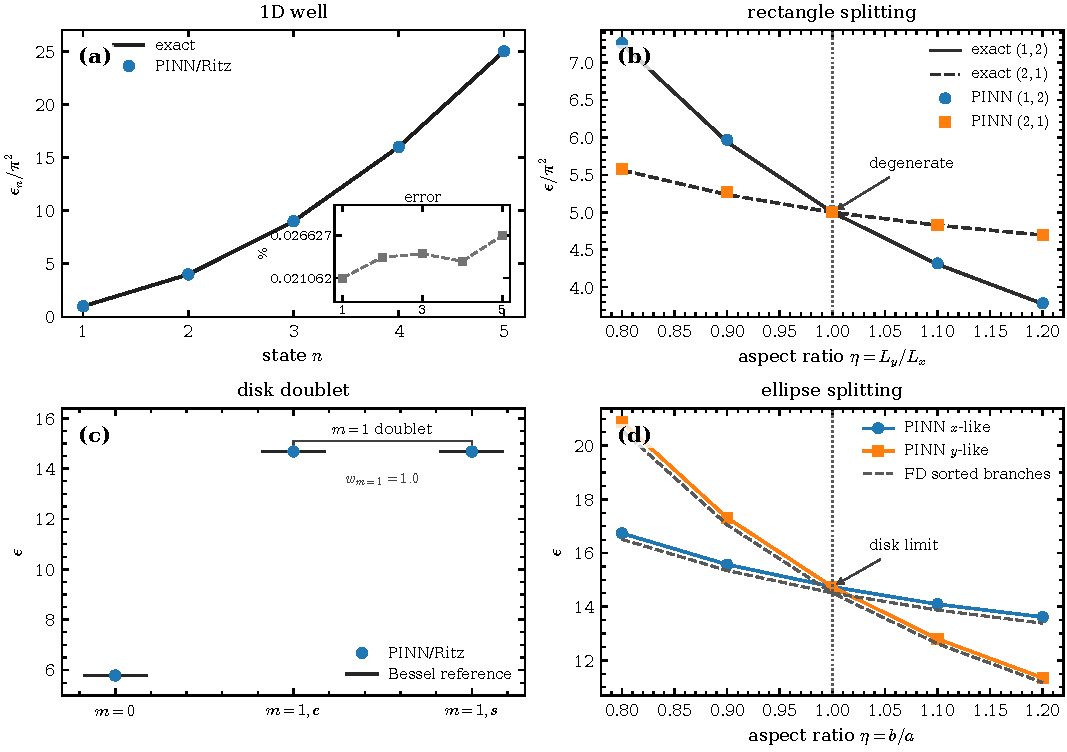
\includegraphics[width=1.0\textwidth]{figures/Fig3_results_summary.pdf}
\caption{Main numerical evidence. Panel (a) shows the one-dimensional excited-state benchmark, where the projected Rayleigh PINN recovers the $n^2\pi^2$ sequence and the correct nodal structure. Panel (b) shows the square-to-rectangle splitting of the $(1,2)/(2,1)$ pair. Panel (c) shows the disk ground state and the $m=1$ doublet. Panel (d) shows the elliptic splitting of the disk doublet into $x$-like and $y$-like branches, compared with an independent finite-difference reference.}
\label{fig:mainresults}
\end{figure}
\FloatBarrier

For the cases with analytical spectra, the reported energy error is the maximum relative eigenvalue error,
\begin{equation}
\delta_\epsilon^{\max}
=
100
\max_i
\left|
\frac{\epsilon_i^{\mathrm{NN}}-\epsilon_i^{\mathrm{ref}}}
{\epsilon_i^{\mathrm{ref}}}
\right|,
\end{equation}
reported in percent. For the ellipse, $\epsilon_i^{\mathrm{ref}}$ is obtained from an independent finite-difference calculation. All eigenvalues are dimensionless, consistent with the Hamiltonian convention $\hat{H}=-\nabla^2$ used throughout this work. Quantities such as nodal count, subspace weight, parity score, and splitting sign are reported as spectral diagnostics rather than as energy units.

\begin{table}[!htbp]
\centering
\caption{Quantitative validation of the main benchmarks. The energy error $\delta_\epsilon^{\max}$ is the maximum relative eigenvalue error, reported in percent. The additional diagnostic column reports the spectral information needed to identify the physical object represented by the learned solution. Eigenvalues and splittings are dimensionless.}
\label{tab:summary}
\small
\renewcommand{\arraystretch}{1.18}
\begin{tabularx}{\textwidth}{@{} l l l >{\raggedright\arraybackslash}X @{}}
\toprule
Case & Reference spectrum & Energy error & Spectral diagnostic \\
\midrule
1D infinite well
&
Analytical
&
$\delta_\epsilon^{\max}=1.6\times10^{-3}\%$
&
Correct nodal count for the first five states: 5/5. \\
Rectangular splitting
&
Analytical
&
$\delta_\epsilon^{\max}=0.743\%$
&
The signed splitting $\Delta_{\rm rect}=\epsilon_{1,2}-\epsilon_{2,1}$ changes sign across $\eta=1$, as expected from the exchange of the compressed direction. \\
Disk doublet
&
Analytical
&
$\delta_\epsilon^{\max}=5\times10^{-4}\%$
&
The learned doublet has unit weight in the analytical $m=1$ subspace, $w_{m=1}=1$. \\
Elliptic splitting
&
Finite difference
&
$\delta_\epsilon^{\max}=1.73\%$
&
The symmetry-adapted branches recover the expected $x$-like and $y$-like parity structure. At the circular limit, the residual splitting is $|E_x-E_y|\approx 6\times10^{-4}$ in dimensionless units. \\
\bottomrule
\end{tabularx}
\end{table}
\FloatBarrier

The signed splittings provide a compact way to read the physics of the deformation. Figure~\ref{fig:deltas} compares the Cartesian and rotational cases using the same diagnostic idea. In both families, the symmetric geometry occurs at $\eta=1$: the square in the rectangular family and the circle in the elliptic family. At this point, the relevant pair of modes is degenerate. When the geometry is deformed away from $\eta=1$, the degeneracy is lifted and the two branches separate.

The sign of the splitting identifies which modal character has become energetically more costly. In the rectangle, this is measured by
$\Delta_{\rm rect}=\epsilon_{1,2}-\epsilon_{2,1}$.
For $\eta=L_y/L_x<1$, the $y$ direction is more compressed, so the $(1,2)$ mode is pushed above the $(2,1)$ mode and $\Delta_{\rm rect}>0$. For $\eta>1$, the compressed direction is exchanged and the sign reverses. In the ellipse, the analogous quantity is $E_y-E_x$: for $\eta=b/a<1$, the $y$-like branch lies higher in energy, while for $\eta>1$ the ordering is reversed. Thus, the sign change across $\eta=1$ is the spectral signature of the exchanged confinement direction.

\begin{figure}[!htbp]
\centering
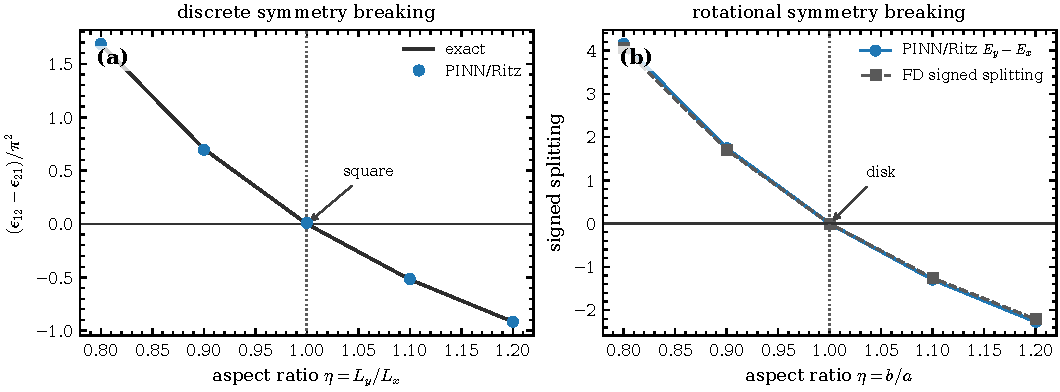
\includegraphics[width=1.0\columnwidth]{figures/Fig4_splitting_deltas.pdf}
\caption{Degeneracy lifting as a sign-changing spectral response. In the rectangle, $\epsilon_{1,2}-\epsilon_{2,1}$ changes sign when the aspect ratio crosses the square geometry. In the ellipse, $E_y-E_x$ changes sign when the aspect ratio crosses the circular geometry. The common pattern is that the branch carrying more variation along the compressed direction shifts to higher energy.}
\label{fig:deltas}
\end{figure}
\FloatBarrier

The previous results show representative trained solutions. We next test whether the same conclusions persist across random initializations. For this purpose, the main cases were repeated over 20 seeds using the formulation associated with each spectral regime. The results are summarized in Table~\ref{tab:ablation}. Here, success is not defined by the same scalar quantity in all rows. For the one-dimensional excited state, success requires the correct energy and nodal count. For degenerate doublets, success requires recovery of the target subspace. For the elliptic splitting, success requires the correct branch ordering and parity character.

One might expect a single well-chosen formulation, tuned once and applied uniformly, to perform reasonably across every regime, since all six rows of Table~\ref{tab:ablation} are variations on the same Rayleigh--Ritz machinery applied to eigenvalue problems of the same Hamiltonian. If that were so, success or failure should track the general quality of the neural architecture and optimizer rather than which spectral object each regime actually calls for. This is not the pattern in Table~\ref{tab:ablation}, since the same subspace-Ritz machinery that is stable for the square and disk doublets (100\% success, subspace weight $w_{\mathcal{S}}\approx1$) is the machinery that fails once used generically for the elliptic splitting (0\% success, mean error $7.1\times10^{2}$), and the same absence of projection that is harmless when the spectrum is already ordered is precisely what allows the one-dimensional $n=5$ state to collapse onto a lower mode (0\% success, mean error $6.3\times10^{1}$). What changes across rows is not the underlying machinery but whether it is matched to the spectral object at hand. This comparison shows why the formulation must follow the spectral object. A state-by-state baseline fails for the fifth one-dimensional state because the optimization can collapse toward a lower-energy mode. The projected Rayleigh formulation removes this lower-state contamination and recovers the ordered excited state. In the square and disk, the subspace Ritz formulation remains stable because it learns the degenerate eigenspace rather than a prescribed basis inside it. In the elliptic case, a generic subspace formulation is unstable because the degeneracy has already been lifted; the appropriate objects are now the two symmetry-labeled branches. The symmetry-sector formulation enforces this structure and recovers the expected branch character across seeds.

\begin{table}[!htbp]
\centering
\caption{Statistical stability of the formulation hierarchy over 20 random initializations. The reported error is the mean relative eigenvalue error in percent. Success is defined by the diagnostic appropriate to each spectral object: energy and nodal count for the one-dimensional excited state, subspace weight for degenerate doublets, and branch ordering/parity for the elliptic splitting.}
\label{tab:ablation}
\scriptsize
\begin{tabularx}{\textwidth}{@{} p{2.4cm} p{2.6cm} c c c p{2.2cm} X @{}}
\toprule
Case & Method & Seeds & Success & Mean energy error (\%) & Diagnostic & Typical outcome \\
\midrule
1D $n=5$ & State-by-state baseline & 20 & 0\% & $6.3\times10^{1}$ & Energy/nodes & Wrong state / energy error \\
1D $n=5$ & Projected Rayleigh & 20 & 100\% & $2.8\times10^{-2}$ & Energy/nodes & Stable excited-state recovery \\
Square doublet & Subspace Ritz & 20 & 100\% & $4.4\times10^{-2}$ & $w_{\mathcal{S}}\approx1$ & Stable degenerate-subspace recovery \\
Disk $m=1$ & Subspace Ritz & 20 & 100\% & $4.3\times10^{-4}$ & $w_{\mathcal{S}}\approx1$ & Stable angular-doublet recovery \\
Elliptic splitting & Generic subspace & 20 & 0\% & $7.1\times10^{2}$ & Parity/order & Branch drift / unstable subspace \\
Elliptic splitting & Symmetry sectors & 20 & 100\% & $1.6$ & Parity $=1$ & Stable branch tracking \\
\bottomrule
\end{tabularx}
\end{table}
\FloatBarrier

For the generic elliptic subspace baseline, the large apparent energy error reflects branch misassignment and unstable parity character, rather than a controlled approximation of the target split branches. In this case, the failure diagnostic is primarily the loss of branch identity.

The state-by-state baseline above shows that a variational formulation can fail when it is not explicitly protected from lower-state contamination. A related but distinct question is whether a strong-form residual formulation, of the kind discussed in the Introduction, can recover the $n=5$ excited state on its own, without the Rayleigh-quotient structure used throughout this paper. One might expect the outcome to depend only on optimization budget: if the residual loss is minimized for long enough, it should eventually settle on the correct eigenpair regardless of where the eigenvalue parameter starts. We tested this directly with a pointwise-residual PINN for the $n=5$ state, in which the eigenvalue $\epsilon$ is itself a trainable parameter alongside the network weights, optimized by minimizing $\int(-\psi''-\epsilon\psi)^2\,dx$ together with a normalization constraint, over three initialization regimes for $\epsilon$: within $5\%$ of the exact $n=5$ energy (informed), within $100\%$ of it (wide), and at the exact energy of the ground state $n=1$ (misleading). Table~\ref{tab:residualcontrol} shows that the outcome tracks the initialization almost exactly, not the optimization budget: with an informed guess, $20/20$ seeds recover the correct nodal count and energy; with a wide but unbiased guess, only $1/20$ do, and the rest scatter across nodal destinations from $n=1$ to $n=9$; and with a misleading guess anchored on the ground state, $20/20$ seeds converge to the $n=1$ nodal structure instead of $n=5$. This is not consistent with residual minimization acting as a free excited-state search: it behaves instead as a local refinement of whichever eigenpair is nearest to the initial guess, which is precisely the prior knowledge that a projected Rayleigh formulation is designed not to need, since it uses no estimate of the target energy at all.

\begin{table}[!htbp]
\centering
\caption{Pointwise-residual PINN for the one-dimensional $n=5$ state under three initialization regimes for the trainable eigenvalue parameter $\epsilon$, 20 seeds each. Success requires both the correct nodal count and a post-hoc Rayleigh energy within tolerance. The nodal destination reports which state index the converged solution actually corresponds to, regardless of success.}
\label{tab:residualcontrol}
\small
\begin{tabularx}{\textwidth}{@{} l c c >{\raggedright\arraybackslash}X @{}}
\toprule
Initialization regime & Success & Mean post-hoc energy error (\%) & Nodal destination across seeds \\
\midrule
Informed ($\pm5\%$ of $\epsilon_5$) & 20/20 & 0.019 & all 20 seeds at $n=5$ \\
Wide ($\pm100\%$ of $\epsilon_5$) & 1/20 & -- & spread over $n=1,\ldots,9$ (Fig.~\ref{fig:residualcontrol}) \\
Misleading (at $\epsilon_1$) & 0/20 & -- & all 20 seeds at $n=1$ \\
\bottomrule
\end{tabularx}
\end{table}
\FloatBarrier

\begin{figure}[!htbp]
\centering
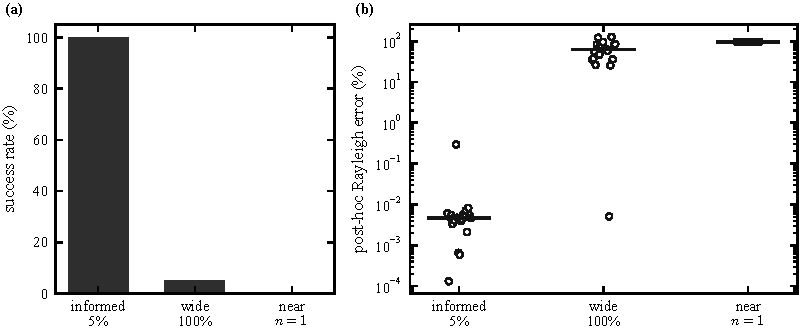
\includegraphics[width=0.92\textwidth]{figures/Fig7_residual_baseline_control.pdf}
\caption{Pointwise-residual PINN for the $n=5$ one-dimensional excited state under three initializations of the trainable eigenvalue parameter. Panel (a) shows the success rate per regime. Panel (b) shows the post-hoc Rayleigh energy error per seed on a log scale: the informed regime clusters near $10^{-3}\%$, the wide regime scatters between roughly $10\%$ and $100\%$, and the misleading regime clusters near $100\%$, consistent with convergence to the wrong state ($n=1$) rather than a partially converged $n=5$ solution.}
\label{fig:residualcontrol}
\end{figure}
\FloatBarrier

The statistical results in Table~\ref{tab:ablation} show that the subspace Ritz formulation is stable for degenerate doublets. The square doublet provides a direct way to inspect what this stability means. In this case, the expected physical object is the two-dimensional eigenspace
\begin{equation}
\mathcal{S}
=
\mathrm{span}\{\psi_{1,2},\psi_{2,1}\}.
\end{equation}
We therefore repeated the square calculation over 50 random initializations and projected the learned modes onto $\mathcal{S}$.

Across the ensemble, the learned doublet remained almost entirely inside $\mathcal{S}$, with subspace weights close to unity and small principal angles relative to the analytical reference. A skeptical reading of what happens next would flag it as a problem: the orientation of the learned basis inside $\mathcal{S}$ varied substantially across seeds, which could easily be mistaken for a failure to converge reproducibly. If the network were simply failing to settle on a stable solution, this variation should appear together with degraded subspace weights or large principal angles, since a poorly converged run would drift outside the target eigenspace as readily as it drifts inside it. This is not what the ensemble shows: subspace weights remain close to unity and principal angles remain small regardless of how the orientation varies, which is exactly the expected behavior for an exactly degenerate eigenvalue, since the Hamiltonian fixes the invariant subspace, but it does not select a unique basis within that subspace. Different learned linear combinations of $\psi_{1,2}$ and $\psi_{2,1}$ therefore represent the same physical eigenspace when they span the same subspace.

This point is important for validation. A one-to-one comparison between individual eigenfunctions would treat internal basis rotations as discrepancies, even though they are physically equivalent. Subspace weights and principal angles remove this ambiguity because they compare the learned object at the level of the eigenspace.

These results clarify how the hierarchy should be validated. In a nondegenerate problem, energy error and nodal count may be sufficient. In a degenerate problem, an almost correct eigenvalue may still correspond to the wrong object if the learned function has insufficient weight in the correct subspace. Conversely, a learned mode may look different from a selected analytical basis and still be physically correct if it lies in the same degenerate eigenspace. The relevant comparison is therefore basis-invariant: it asks whether the learned function or learned Ritz space lies in the correct invariant subspace. After deformation, the diagnostic changes again, because the formerly degenerate pair becomes two distinguishable symmetry branches. The diagnostic must therefore match the spectral object: nodal structure for ordered states, subspace weight for degenerate eigenspaces, parity for symmetry-split branches, and modal overlap for near-degenerate continua.

The subspace diagnostic used here can be written as
\begin{equation}
w_{\mathcal{S}}(\psi)
=
\sum_{j\in\mathcal{S}}
|\langle \psi,\psi_j^{\mathrm{ref}}\rangle|^2,
\end{equation}
where $\mathcal{S}$ denotes the reference degenerate eigenspace. This quantity is insensitive to arbitrary rotations of the basis inside the degenerate space. Principal angles provide the corresponding basis-invariant language for comparing two computed subspaces \cite{DavisKahan1970,KnyazevArgentati2002}. For the ellipse, the corresponding diagnostic also includes the parity character and the sign of $E_y-E_x$. Figure~\ref{fig:hierarchy} summarizes this logic.

\begin{figure}[!htbp]
\centering
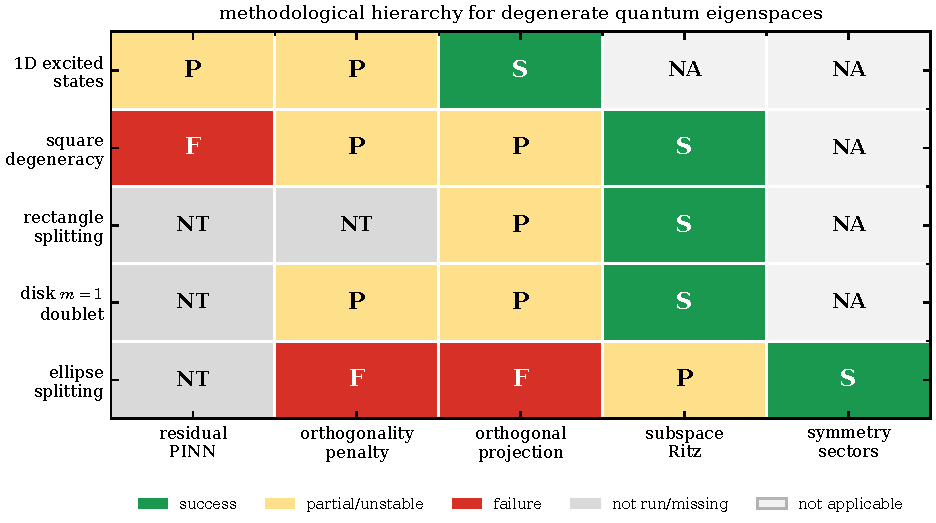
\includegraphics[width=0.92\textwidth]{figures/Fig2_method_ablation.pdf}
\caption{Formulation hierarchy for neural quantum eigensolvers. Each row corresponds to a spectral regime and each column to a possible variational strategy. The figure shows how the appropriate formulation changes with the physical object being represented: orthogonal projection for ordered excited states, subspace Rayleigh--Ritz training for degenerate eigenspaces, and symmetry-adapted sectors for branches split by residual reflection symmetries. Cell color and symbol indicate success (green), partial or unstable behavior (yellow, $\pm$), failure (red, $\times$), not run or missing (gray, $?$), or not applicable (hatched, $-$). The residual-PINN entry for the one-dimensional excited state is marked partial rather than a flat failure: as Table~\ref{tab:residualcontrol} and Figure~\ref{fig:residualcontrol} show, this formulation recovers the $n=5$ state only when the eigenvalue parameter is initialized close to the target energy, and otherwise collapses onto a different nodal count.}
\label{fig:hierarchy}
\end{figure}
\FloatBarrier

\subsection{Near degeneracies and modal tracking}

The previous examples involve exact degeneracies or degeneracy lifting that can still be labeled by residual symmetry. The avoided crossing considered here is a qualitatively richer final test. Along the deformation path, two branches approach each other, interact, and exchange modal character. The ordered eigenvalue index remains well defined, but it does not by itself identify which physical mode is being followed. In this regime, branch identity is more naturally read from modal overlaps.

We construct the avoided crossing from the rectangular $(1,2)$ and $(2,1)$ branches, which cross at $\eta=1$ in the unmixed problem. A controlled mixing potential is added,
\begin{equation}
V(u,v)=
\lambda_{\mathrm{mix}}
\left(u-\frac{1}{2}\right)
\left(v-\frac{1}{2}\right),
\label{eq:mixing}
\end{equation}
with a nonzero matrix element between $\psi_{1,2}$ and $\psi_{2,1}$. This coupling opens a finite gap and produces the standard two-level level-repulsion mechanism associated with avoided crossings and Landau--Zener-type mixing \cite{VonNeumannWigner1929,Zener1932}. The gray curves in Fig.~\ref{fig:avoided} correspond to the unmixed rectangular energies of $H_0(\eta)$,
\begin{equation}
E_{n_x,n_y}^{(0)}(\eta)
=
\pi^2
\left(
n_x^2+\frac{n_y^2}{\eta^2}
\right),
\end{equation}
whereas the black curves are a sine-basis spectral reference for the coupled Hamiltonian $H_0(\eta)+V_{\rm mix}$. This reference is obtained by diagonalizing the coupled Hamiltonian in a truncated rectangular sine basis with $1\le n_x,n_y\le 10$. Increasing the truncation to $12\times12$ and $14\times14$ modes changed the two near-degenerate reference branches by less than $0.09\%$ and $0.18\%$, respectively, over the sampled deformation path.

For this test, we use the carrier-assisted Rayleigh--Ritz formulation in Eq.~(\ref{eq:carrier}). The carriers define the near-degenerate spectral space associated with $\{\psi_{1,2},\psi_{2,1}\}$. For $\alpha=0$, the calculation reduces to a fixed two-mode Ritz problem. For $\alpha>0$, the carrier modes are augmented by boundary-preserving neural corrections. In the latter case, the correction is treated as a regularized perturbation of the carrier space, using an $H^1$-type penalty to control both the amplitude and the derivative content of the neural correction. This regularization is needed because an unconstrained variational correction can lower the Rayleigh quotient by drifting away from the intended near-degenerate band.

The branch identity is measured by the modal weights
\begin{equation}
w_{12}=|\langle\psi,\psi_{1,2}\rangle|^2,
\qquad
w_{21}=|\langle\psi,\psi_{2,1}\rangle|^2.
\end{equation}
With $\alpha=0.05$ and regularized neural corrections, the carrier-assisted calculation follows the avoided crossing over the full deformation path. The regularization was introduced precisely because an unconstrained correction could lower the Rayleigh quotient by drifting away from the intended near-degenerate band rather than by improving the representation of $\psi_{1,2}$ and $\psi_{2,1}$; had that drift dominated, one would expect either a large energy error or a poorly conditioned mass matrix, or both, and neither is observed, since the maximum relative energy error is approximately $1.35\%$, and the Ritz mass matrix remains well conditioned, with condition numbers close to unity. The modal weights confirm that the correction tracked the physical band rather than an artifact of the optimization, since the lower branch starts predominantly with $(2,1)$ character for $\eta<1$, becomes an approximately equal mixture near $\eta=1$, and emerges with predominantly $(1,2)$ character for $\eta>1$.

\begin{figure}[!htbp]
\centering
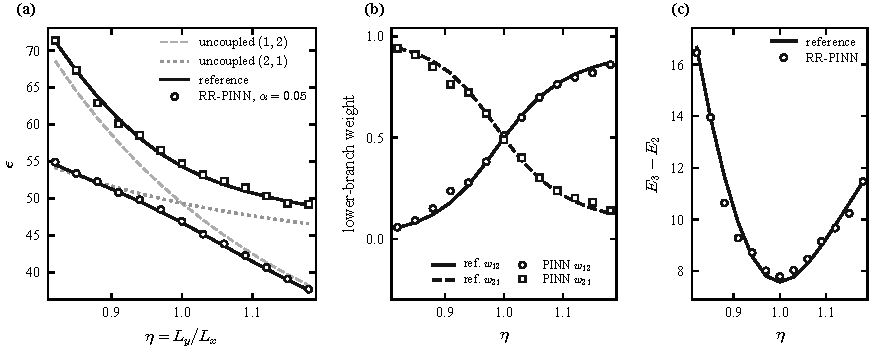
\includegraphics[width=0.98\textwidth]{figures/Fig5_avoided_crossing_modal_tracking.pdf}
\caption{Modal tracking in a controlled avoided crossing. A weak mixing potential couples the rectangular $(1,2)$ and $(2,1)$ modes and opens a finite gap near $\eta=1$. The carrier-assisted Rayleigh--Ritz calculation with $H^1$-regularized neural corrections, using $\alpha=0.05$, follows the avoided gap and the exchange of lower-branch modal character through the weights $w_{12}$ and $w_{21}$. The maximum relative energy error over the deformation path is approximately $1.35\%$.}
\label{fig:avoided}
\end{figure}
\FloatBarrier

A natural objection to the previous test is that the coupling between $\psi_{1,2}$ and $\psi_{2,1}$ was introduced through an added potential $V(u,v)$ rather than through the geometry itself, which is not the same mechanism used everywhere else in this paper. If the avoided crossing depended specifically on that potential, it would not really belong to the geometric-symmetry-breaking picture developed for the square, rectangle, disk, and ellipse, and the title's claim would not extend to this last case. We therefore repeated the calculation with the mixing potential removed and the coupling generated purely by a geometric deformation: a shear of the rectangular domain, $x=u+\gamma v$, $y=\eta v$, with $\gamma=0.18$ fixed and $\eta$ swept as before. The shear introduces a cross term $g_{12}=-\gamma/\eta^{2}$ in the metric of the Laplacian, which mixes $\psi_{1,2}$ and $\psi_{2,1}$ without any potential term, and the same carrier-assisted Rayleigh--Ritz construction of Eq.~(\ref{eq:carrier}) is used unchanged, with the metric factors of the sheared domain entering the stiffness matrix in place of $V(u,v)$. An independent sine-basis spectral reference was recomputed for the sheared metric. The result is the same qualitative phenomenology as Fig.~\ref{fig:avoided}: the reference gap $E_3-E_2$ reaches a nonzero minimum of $5.21$ at $\eta=1$ rather than closing to zero, the carrier-assisted calculation follows this gap with a maximum relative energy error of $1.08\%$ and a Ritz mass matrix conditioned below $1.0004$ throughout, and the lower-branch modal weights exchange character across $\eta=1$ in the same way as in the potential-driven case (Fig.~\ref{fig:avoidedgeom}). This confirms that the avoided crossing and the associated modal-overlap diagnostic are generic consequences of a geometric coupling, consistent with the rest of this paper, and not an artifact specific to the added potential used in the first construction.

\begin{figure}[!htbp]
\centering
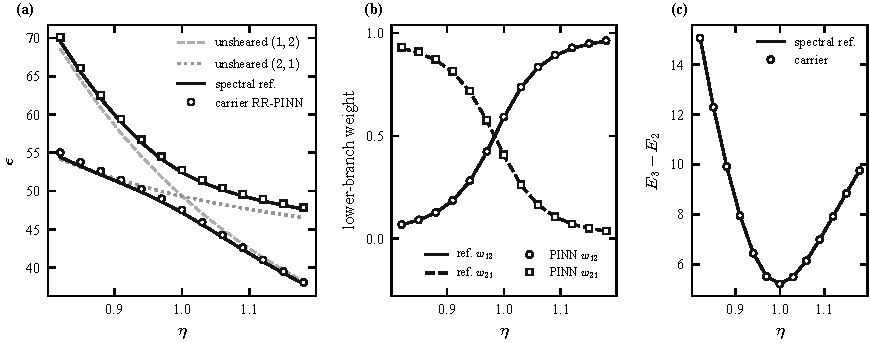
\includegraphics[width=0.98\textwidth]{figures/Fig6_avoided_crossing_geometric.pdf}
\caption{Avoided crossing generated by a purely geometric coupling. The rectangular domain is sheared as $x=u+\gamma v$, $y=\eta v$ with $\gamma=0.18$, which mixes the $(1,2)$ and $(2,1)$ modes through the cross term of the metric rather than through an added potential. Panel (a) shows the unsheared uncoupled energies (gray) against the sheared spectral reference and the carrier-assisted Rayleigh--Ritz calculation. Panel (b) shows the exchange of lower-branch modal weight across $\eta=1$. Panel (c) shows the reference and computed gap $E_3-E_2$, which stays bounded away from zero at $\eta=1$, as expected for an avoided crossing.}
\label{fig:avoidedgeom}
\end{figure}
\FloatBarrier

This result extends the same diagnostic logic to a setting where symmetry labels are no longer sufficient. In asymmetric domains, such as a scalene triangle or an irregular polygon, split branches cannot generally be classified by parity. Along a geometric path parametrized by $\eta$, branch identity should instead be followed through neighboring-state overlaps,
\begin{equation}
O_{ij}(\eta,\eta+\Delta\eta)
=
|\langle \psi_i(\eta),\psi_j(\eta+\Delta\eta)\rangle|^2,
\end{equation}
or, for nearly degenerate groups, through principal angles between subspaces \cite{KnyazevArgentati2002}. The avoided-crossing test therefore gives a controlled example of the continuation strategy that would be needed in less symmetric geometries.

The present calculations were designed as controlled spectral tests rather than optimized production solvers. Classical finite-difference, finite-element, spectral, and Rayleigh--Ritz methods remain more efficient for these low-dimensional reference domains. The value of the neural formulation in this setting is its ability to combine boundary satisfaction, variational structure, orthogonality, subspace representation, symmetry-sector constraints, and modal tracking in a single differentiable framework.

A limitation of the present study is that the domains are idealized infinite wells. This choice isolates the spectral consequences of symmetry and deformation, while realistic quantum dots may involve finite barriers, smooth confinement potentials, effective-mass discontinuities, magnetic fields, and many-body interactions. These extensions require additional validation, while preserving the central diagnostic principle developed here, namely that the neural eigensolver should be assessed against the spectral object selected by the physics.

\section{Conclusions}

We developed a Rayleigh--Ritz physics-informed neural formulation for confined quantum eigenproblems in geometry-parametrized domains. The study was organized around a sequence of spectral regimes in which the relevant object changes from ordered eigenstates to degenerate eigenspaces, symmetry-split branches, and near-degenerate bands. This organization makes the role of the variational representation explicit: each regime requires a formulation and a validation diagnostic consistent with the spectral structure selected by the Hamiltonian.

For ordered excited states, explicit projection against lower eigenspaces stabilizes the Rayleigh minimization and recovers the correct nodal structure. For degenerate square and disk spectra, the subspace Rayleigh--Ritz formulation recovers the invariant eigenspace without imposing a particular basis inside it. Under rectangular and elliptic deformations, the lifted branches are followed through signed splittings and symmetry-adapted sectors. In the avoided-crossing test, the carrier-assisted formulation with regularized neural corrections tracks both the avoided gap and the exchange of modal character, showing that modal overlap is the appropriate diagnostic near quasi-degeneracy. This avoided-crossing phenomenology is not an artifact of the specific coupling used to generate it: a purely geometric shear reproduces the same gap and modal exchange without any added potential, confirming that the mechanism is generic to geometric coupling rather than tied to the added potential used in the first construction. A controlled initialization test of a pointwise-residual formulation further shows that residual minimization recovers the correct excited state only when it starts from a near-exact energy guess, collapsing onto the wrong state otherwise; the projected Rayleigh formulation used throughout this paper requires no such guess. Taken together, these results support a spectral-object viewpoint for neural eigensolvers of Hermitian operators, since energy accuracy, nodal count, subspace weight, parity character, branch splitting, and modal overlap play complementary roles as the spectral structure changes.

The present benchmarks use idealized infinite-well domains so that the effects of symmetry, degeneracy, and geometric deformation can be isolated cleanly. The same framework can be extended to three-dimensional degeneracies, asymmetric domains without residual parity labels, finite barriers, smooth confinement potentials, effective-mass variations, magnetic fields, and more realistic quantum-dot Hamiltonians. These extensions will require additional numerical validation, especially when analytical spectra are no longer available, while preserving the central diagnostic principle developed here, namely that the learned solution should be assessed at the level of the spectral object represented by the physics.

\section*{Code availability}

The code and data needed to reproduce the results will be made available in a public GitHub repository at \url{https://github.com/lvitoria}.

\section*{Acknowledgments}



\bibliographystyle{iopart-num}
\bibliography{references}

\end{document}
